\subsubsection{الگوی \lr{Five Layer}}
\label{arch5LayerSec}
\begin{RTL}
الگوی معماری پنج‌لایه \cite{ref4} یک تطبیق
خاص از \nameref{archLayerSec} است
که برای ساختاردهی بسیاری از سیستم‌های نهفته و بی‌درنگ
مفید است. این الگو معماری منطقی را به پنج لایه
تقسیم می‌کند که این امر به توسعه‌دهندگان کمک می‌کند
تا به راحتی ساختار سیستم‌های جدید را درک کنند.
این الگو از قابلیت انتقال بین پلتفرم‌های مختلف پشتیبانی
می‌کند و یک پلتفرم انتزاعی فراهم می‌کند که تطبیق برنامه‌ها
را آسان‌تر می‌سازد. در حالی که این الگو بسیاری از
مزایای \nameref{archLayerSec} را دارد، از جمله کارایی بالا به دلیل تعداد
کم لایه‌ها، ممکن است برای تجزیه کافی سیستم‌های پیچیده مناسب نباشد.
\end{RTL}
\begin{figure}[h!]
\centering
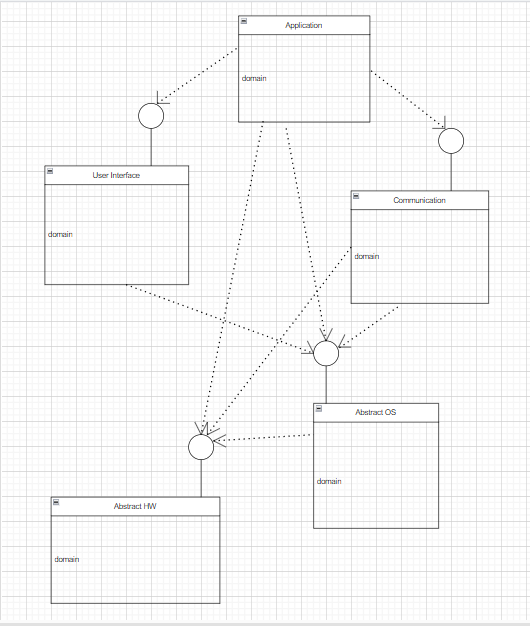
\includegraphics[scale=0.75]{images/first/5layer.png}
\caption{ساختار الگوی \lr{Five Layer}}
\end{figure}